\documentclass[10pt,letterpaper,twocolumn]{article}
% \usepackage[twocolumn]{geometry}
\usepackage{lmodern}% http://ctan.org/pkg/lm

% use Unicode characters - try changing the option
% if you run into troubles with special characters (e.g. umlauts)
\usepackage[utf8x]{inputenc}
% clean citations
\usepackage{cite}
% hyperref makes references clicky. use \url{www.example.com}
% or \href{www.example.com}{description} to add a clicky url
\usepackage{nameref}
% line numbers
\usepackage[right]{lineno}
% improves typesetting in LaTeX
% \usepackage{microtype}
% degree symbol
\usepackage{gensymb}
\usepackage{amsmath}
\usepackage{booktabs}
% use adjustwidth environment to exceed text width (see examples in text)
\usepackage{changepage}
% adjust caption style
\usepackage[aboveskip=1pt,labelfont=bf,
            labelsep=period,singlelinecheck=off]{caption}
% remove brackets from references
\makeatletter
\renewcommand{\@biblabel}[1]{\quad#1.}
\makeatother

% headrule, footrule and page numbers
\usepackage{lastpage,fancyhdr,graphicx}
\usepackage{epstopdf}
\pagestyle{myheadings}
\pagestyle{fancy}
\fancyhf{}
\rfoot{\thepage/\pageref{LastPage}}
\renewcommand{\footrule}{\hrule height 2pt \vspace{2mm}}
% \fancyheadoffset[L]{2.25in}
% \fancyfootoffset[L]{2.25in}
% use \textcolor{color}{text} for colored text (e.g. highlight to-do areas)
\usepackage{color}
% define custom colors (this one is for figure captions)
\definecolor{Gray}{gray}{.25}
% this is required to include graphics
\usepackage{graphicx}
% set the figures directory
\graphicspath{{./figs/}}
% use if you want to put caption to the side of the figure - see example in text
\usepackage{sidecap}
% \usepackage[urlcolor  = blue]{hyperref}

% hyperurls packages:
\usepackage{xcolor}
\usepackage[colorlinks = true,
            linkcolor = blue,
            urlcolor  = blue,
            citecolor = blue,
            anchorcolor = blue]{hyperref}

% use for have text wrap around figures
\usepackage{wrapfig}
\usepackage[pscoord]{eso-pic}
\usepackage[fulladjust]{marginnote}
\reversemarginpar{}

% new commands
\newcommand{\cel}{\emph{C.~elegans}}
\newcommand{\fog}{\emph{\mbox{fog-2}}}
\newcommand{\ecol}{\emph{E.~coli}}
\newcommand{\hobesity}{957}
\newcommand{\wobesity}{614}
\newcommand{\hlupus}{283}
\newcommand{\wlupus}{135}
\newcommand{\harthritis}{309}
\newcommand{\warthritis}{124}

\newcommand{\qval}[1]{\ensuremath{q<10^{-#1}}}

% more space between rows
\newcommand{\ra}[1]{\renewcommand{\arraystretch}{#1}}

\title{
  \Large
  \textbf{
  % Phenotype Enrichment Discovers Phenologs for Disease Modeling in \cel{}
  Phenotype and gene ontology enrichment as guides for disease modeling
  in \cel{}
          }
}

\author{David Angeles-Albores\textsuperscript{1}
\and{}
Raymond YN Lee\textsuperscript{1}
\and{}
Juancarlos Chan\textsuperscript{1}
\and{}
Paul W Sternberg\textsuperscript{1,*}
}

\begin{document}

% \vspace*{0.35in}

% title goes here:
\twocolumn[
% title
\maketitle

\textbf{1} Department of Biology and Biological Engineering,
and Howard Hughes Medical Institute, Caltech, Pasadena, CA, 91125, USA\\
\textbf{*} Corresponding author. Contact:pws@caltech.edu

\section*{Abstract}
\bf{}
Genome-wide experiments have the capacity to generate massive amounts of unbiased
data about an organism. In order to interpret this data, dimensionality reduction
techniques are required. One approach is to annotate genes using controlled languages
and to test experimental datasets for term enrichment using probabilistic methods.
Although gene, phenotype and anatomy ontologies exist for \cel{}, no unified
software offers enrichment analyses of all the ontologies using the same methodology.
Here, we present the WormBase Enrichment Suite, which offers users the
ability to test all nematode ontologies simultaneously. We show that
the WormBase Enrichment Suite provides valuable insight into different
biological problems. Briefly, we show that phenotype enrichment analysis (PEA) can
help researchers identify disease phenologs, phenotypes that are homologous across species,
which can inform disease modeling in \cel{}. The WormBase Enrichment Suite
analysis can also shed light on RNA-seq datasets by showing what
molecular functions are enriched, which phenotypes these functions are implicated
in and what tissues are overrepresented in the dataset. Finally, we explore the
phenotype-anatomy relationship, showing that a small subset of highly specific
tissues are disproportionately likely to cause an Egl phenotype, but inferring
tissue expression from an Egl phenotype is limited to the largest tissues.
]


% now start line numbers
\nolinenumbers{}

\section*{Introduction}
The last decade has seen an explosion of techniques capable of genome-wide
measurements. Some examples of genome-wide tools include
RNA-seq~\cite{Mortazavi2008} to measure gene expression or
CHIP-seq~\cite{Johnson2007} to measure protein binding to chromatin. These tools are capable
of generating large quantities of data. Understanding these data, and generating
hypotheses from them remains challenging. A common approach used to understand
these datasets is to reduce the dimensionality of the data via enrichment
analyses of ontologies~\cite{TheGeneOntologyConsortium2000a}, which helps
researchers understand what terms are
overrepresented beyond random levels. By analyzing overrepresented terms in
aggregate, researchers can better understand what biological processes were most
affected in a given experiment, and form hypotheses about what is
happening~\cite{Rhee2008}.
This approach is limited by what ontologies can be tested for enrichment.
The best-known ontology for biological research is the Gene Ontology (GO), which
provides a controlled language to describe molecular and cellular functions of
genes~\cite{TheGeneOntologyConsortium2000a}.
In \cel{}, gene, tissue and phenotype ontologies exist
% which provide
% controlled languages
with which to describe \cel{} anatomy and phenotypes
respectively~\cite{Schindelman2011,Lee2003}. These ontologies are curated by
professional curators at WormBase, which is a repository of all \cel{}
data~\cite{Howe2016}.
However, enrichment tools
only exist for gene and tissue ontologies
in the community today (see for example~\cite{Chikina2009,Mi2013,Angeles-Albores2016}).
Another limitation is that
tissue enrichment testing is not offered on the same websites as GO enrichment
testing, which requires users to test their data on different websites that may
or may not use different methodologies to detect enrichment.

Another way to use enrichment tools is for evolutionary comparison purposes.
In molecular biology it is often useful to know when a gene is homologous
between two species---that is to say, common by descent---because knowledge of
homology often brings with it knowledge of function. Indeed, many
important gene regulatory networks (GRNs) are conserved between organisms as
highly diverged as nematodes and humans (for example, see~\cite{Sternberg1998}).
While genes and GRNs may be conserved between species, their outputs often differ.
For example, the gene Pax6 (Eyeless in \emph{Drosophila melanogaster})
is involved in eye formation in humans and fruit-flies~\cite{Quiring1994}. Although
nematodes have conserved this gene, they do not have eyes~\cite{Zhang1995,Chisholm1995}.
The concept of a phenolog has been put forward to explain relationships between
phenotypes that have the same underlying genetic
regulatory network~\cite{McGary2010,Lehner2013}.
Formally, two phenotypes are phenologs of each other if the orthologs of the
genes that cause a phenotype in an organism cause a second phenotype in another.

To study a clinically relevant disease in a non-human, an appropriate
model has to be established. A straightforward method towards establishing a
disease model in
\cel{} is to link a disease to a causal gene, then to identify the homologous
gene in \cel{} and then to study the function of the genetic homolog to
extrapolate back to humans. However, this method relies on the existence of
known disease genes and requires that the homolog have a phenotype that can be
reliably identified and studied. A fundamentally different way to establish a
disease model in \cel{} would be to identify the phenologs of the disease to be
studied in \cel{} by identifying disease-associated human genes in an unbiased
manner through genome-wide association studies (GWAS) and identified candidate
homolog genes in \cel{}. The orthologs can be used to identify \cel{} disease
phenologs, which can in turn be used as the basis for screens to identify
genes that are associated with that phenolog. Approaches similar to this have
been successfully used in the past to make non-obvious links between phenotypes
in different species~\cite{McGary2010}.

The concept of a phenolog can also be useful when applied within a species.
In \cel{}, not all phenotypes are equally easy to study. Although genome-wide
measurements can help elucidate the genetic network underlying a phenotype,
devising screens to test which genes are functionally important can be difficult.
A common strategy to study phenotypes that are difficult to screen is to
select an easier-to-screen phenolog, and to test positive hits for the true
phenotype of interest afterwards. For example, candidate genes to extend the \cel{}
lifespan can be first screened for using heat shock survival
genes involved in \cel{} aging
sensitivity can be identified using stress assays~\cite{Kim2007a,Mehta2009}.
Currently, selection of screening phenotypes is performed based on researcher
experience. By formalizing phenotype enrichment analysis as a tool with which to
analyze gene sets, researchers should be able to formally establish phenologs,
which has consequences for screen design.
% eating defects in an ablated strain

An additional problem with genome-wide
queries of \cel{} states (be they developmental, such as
L1, L2, dauer; behavioral states such as awake versus asleep; or other) is that
they do not
always have a straightforward interpretation in terms of phenotypes. In these
situations, researchers must rely on intuition to select a phenotype for which to
screen. As a result, many hits may go unexplored that would prove fruitful. The
question of how to design a screen that is maximally informative is an important
question that has so far not been addressed within this community.

To facilitate understanding of large datasets, and to make discovery of
phenologs easier, we have completed an enrichment tool suite in WormBase
that allows users to rapidly perform phenotype, tissue and gene ontology
enrichment analyses (PEA, TEA and GEA respectively) on curated \cel{} ontologies
using the same methodology for each one.
% They are located at
% % TODO: include links.
We applied our tools towards the unbiased discovery of phenologues of
multigenic, complex diseases including
% Diseases to study:
systemic lupus erythematosus, obesity and obesity-related traits,  and
rheumatoid arthritis
by using genes associated with these
diseases via genome-wide association studies. We illustrate the utility of
the complete enrichment suite for finding new relationships in complex data by
analyzing a ciliary neuron transcriptome~\cite{Wang2015}. Finally, we show that
the dictionaries generated for these enrichment analyses can help elucidate the
contributions of specific tissues to specific phenotypes.

\section*{Methods}
\subsection*{Implementing the enrichment analyses}
All scripts were implemented in Python 3.5~\cite{Rossum2011}. We used
pandas~\cite{McKinney2011} and scipy~\cite{Oliphant2007} to write the
statistical testing framework. Matplotlib~\cite{Hunter2007} and Seaborn~\cite{Waskom}
libraries are used to generate all plots. Testing was performed using the
WormBase version WS256. The WormBase Enrichment suite can be installed using
pip via the command:

\texttt{pip install tissue\_enrichment\_analysis}

% A brief tutorial on how to use the command line tool can be found in the SI.
% A brief tutorial on how to interact with the suite using python is available
% as a Jupyter notebook~\cite{Perez2007} in the SI.

\subsection*{Human disease phenolog identification}
We used the GWAS EBI-NHGRI catalog~\cite{MacArthur2016} to extract information
on all genome-wide
association studies deposited there. We only selected traits that had $>300$
associated genes. We identified 24 traits that met our criteria. Next, we used
DIOPT~\cite{Hu2011} to identify candidate orthologs for the genes associated with these
traits. Briefly, DIOPT combines a large number of methods for identifying orthologs
and returns homolog candidates associated with a compound score. Depending on the score,
orthologs can be considered `high', `moderate' or `low' rank, reflecting confidence
in the homology. Many-to-one and one-to-many homology relationships are allowed
in DIOPT, reflecting a mixture of uncertainty and family expansion/reduction.
For our study, we only accepted homolog candidates with `high' or `moderate' scores
and we did not insist on a one-to-one relationship between genes.

\begin{figure}[htbp]
  \renewcommand{\familydefault}{\sfdefault}\normalfont{}
  \centering
  \includegraphics[width=\linewidth]{gwas-design.pdf}
  \caption{Experimental design for human-nematode phenologue identification.
           We used GWAS candidates from the EBI-NHGRI catalog to identify
           disease associated genes, then used DIOPT to identify candidate
           orthologs in \cel{}. Orthologs were used to run phenotype, gene
           and tissue ontology enrichment analyses to identify disease
           phenologues.}
\label{fig:gwas}
\end{figure}


After we identified worm orthologs for each trait, we reassessed how many traits
still had $>100$ gene candidates, and dropped all traits that had less than this
for our analysis. We identified 18 traits that met this criteria. The gene
lists for each of these 18 traits were then analyzed for gene, tissue and
phenotype enrichment (see~Fig.\ref{fig:gwas}). Tissue enrichment was
performed using the WormBase Tissue Enrichment Analysis (TEA)
tool~\cite{Angeles-Albores2016}.


\section*{Results}
\subsection*{Developing the WormBase enrichment suite}
% TODO add numbers instead of XXX
We developed the dictionaries for PEA and GEA using the same procedure as was
used for TEA~\cite{Angeles-Albores2016}. We generated a dictionary that
included terms with at
least 50 annotating genes or more and had a similarity threshold of 0.95 for PEA
(the total number of terms in the dictionary was 251, annotated by 9,169 genes
 for the version WS256);\@ and we generated a
dictionary that included terms with at least 50 annotating genes or more and
had a similarity threshold of 0.95 for GEA (the total number of terms in this
dictionary is 271, annotated by 14,636 genes for the version WS256).
\@ Next, we benchmarked the dictionaries on the same gene
sets as TEA and obtained enrichment of all the expected
categories~\cite{Gaudet2004a, Spencer2011, Cinar2005, Watson2008a,
Pauli2006, Portman2004, Fox2007, Smith2010}.
For example,
on a gene set enriched for embryonic muscle genes~\cite{Watson2008a},
the top two enriched
phenotype terms by q-value were `muscle system morphology variant' and `body
wall muscle thick filament variant'; the top two enriched GO terms were
`myofibril' and `striated muscle dense body'. For all the benchmarking
results, see supplementary information. Having generated and validated our
dictionaries, we proceeded to identify phenologs for several common human
diseases.

\subsection*{Applying the WormBase enrichment suite}
To discover phenologs, we first needed to identify genes that
contribute to a disease in an unbiased manner. One way to discover gene
associations in an unbiased manner is to perform GWSA in human populations.
Therefore, we used the GWAS NHGRI-EBI
Catalog~\cite{MacArthur2016} to identify genes associated with human diseases. We found the
best nematode candidate orthologs for these genes using DIOPT~\cite{Hu2011} and applied
our enrichment suite to each of these gene regulatory networks.

\subsection*{Systemic lupus erythematosus}
Systemic lupus is an autoimmune disease that is believed to be polygenic in
nature~\cite{Mohan2015}. It mainly affects women and is characterized by painful
and swollen joints, hair loss, and fatigue~\cite{Lisnevskaia2014}. Since worms do not have a
cellular immune system, we were interested in what phenologs corresponded to
this disorder in \cel{}. To establish phenolog candidates, we obtained
\hlupus{} genes associated with the disease via GWAS studies, and found
\wlupus{} homolog candidates in \cel{}.

Lupus-associated orthologs were reasonably well annotated. Slightly more than half
of the genes had at least one phenotype annotation ($76/\wlupus{}$) and almost
all genes were annotated to at least one tissue or gene ontology term
($104/\wlupus{}$ and $115/\wlupus$ genes respectively).
We found that Lupus-associated orthologs were enriched in `aneuploidy' (7 genes,
\qval{1}) and `meiotic chromosome segregation' (8 genes, \qval{1}). `Cell fate
transformation' (6 genes, \qval{1}), and `excess intestinal cells'
(5 genes, \qval{1}) were also overrepresented, as was `male tail morphology'
(6 genes, \qval{1}). Finally, the phenotype `nonsense mRNA accumulation' was also
enriched (5 genes, \qval{1}) (see Fig.~\ref{fig:lupus}).

\begin{figure}[htbp]
  \renewcommand{\familydefault}{\sfdefault}\normalfont{}
  \centering
  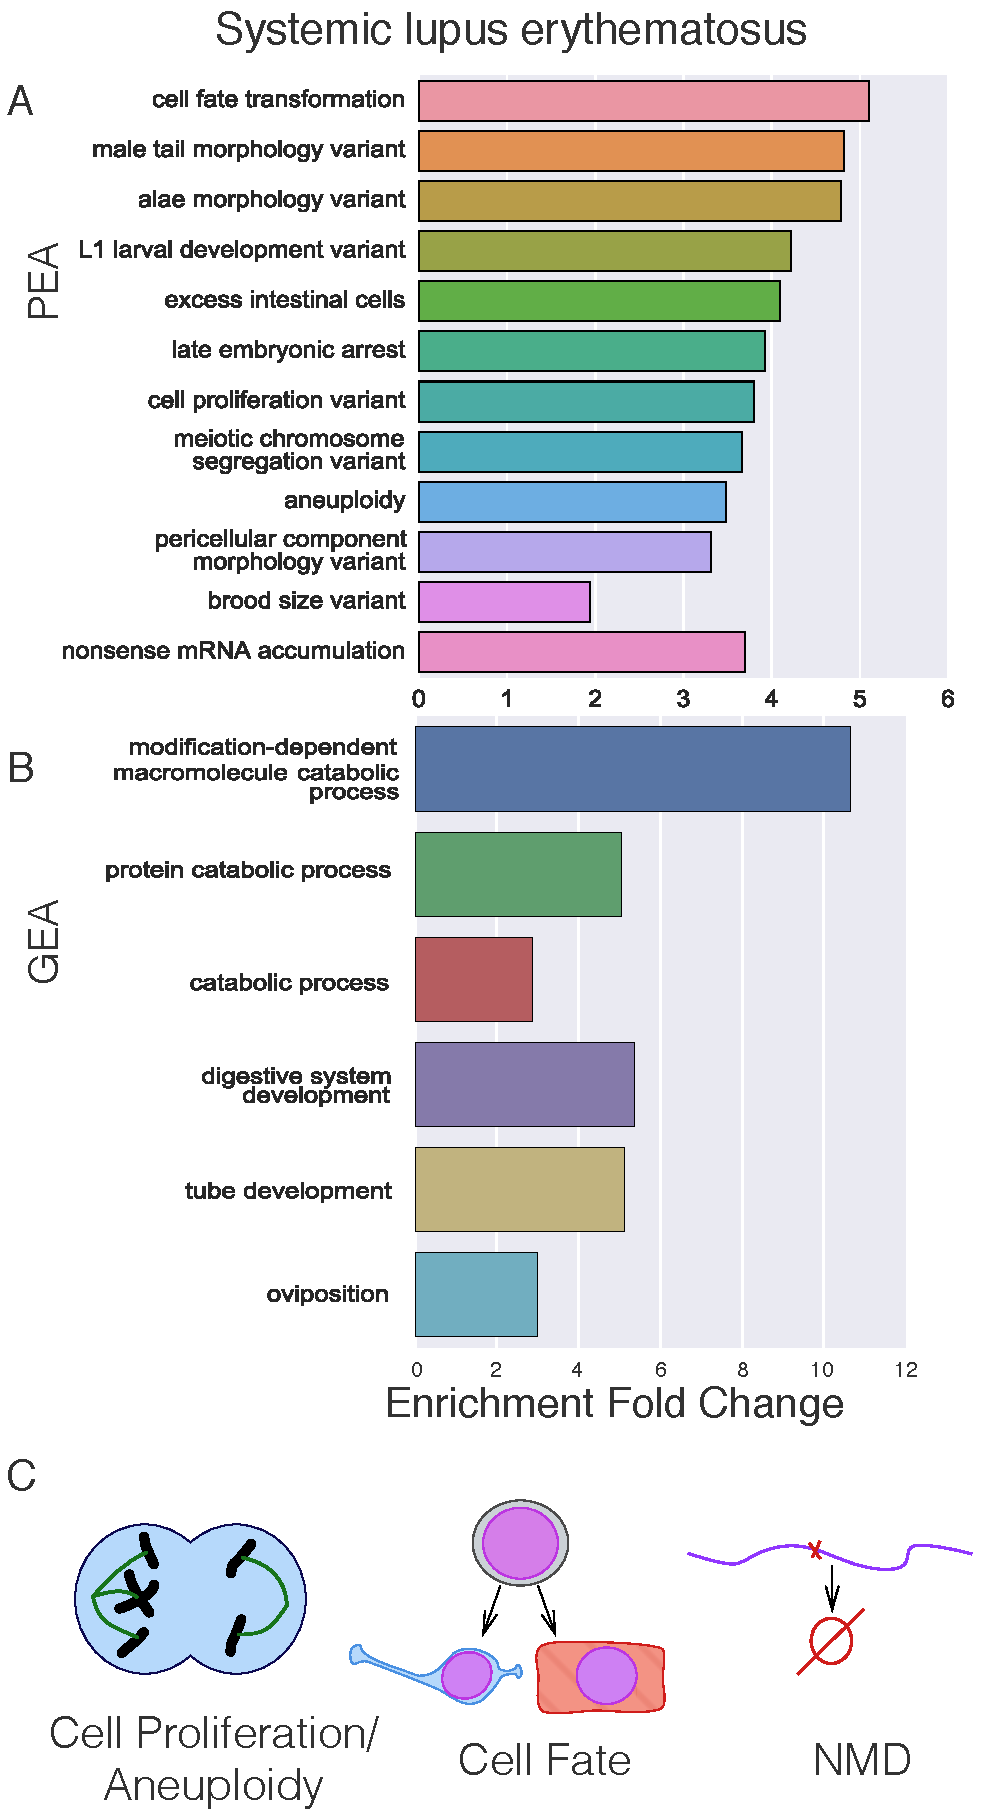
\includegraphics[width=\linewidth]{systemic-lupus.pdf}
  \caption{Phenologue identification for systemic lupus erythematosus.
           \textbf{A} Phenotype Enrichment Analysis. \textbf{B} GO Enrichment
           Analysis. \textbf{C} Lupus in \cel{} may be best represented by
           a combination of three phenotypes: Cell proliferation possibly
           accompanied by aneuploidy; cell fate transformations that may lead
           to dysmorphias; and a molecular phenotype involving impairment of
           the Nonsense-Mediated Decay (NMD) pathway.}
\label{fig:lupus}
\end{figure}

TEA suggested that the
`excretory duct cell' (5 genes, \qval{2}) and the `posterior gonad arm' are
overrepresented in this dataset. We also found that the Pn.p cells P3.p through
P8.p were enriched in this dataset (5 genes, \qval{1}). GO enrichment pointed
at `modification-dependent macromolecule catabolic process' (23 genes,
\qval{15}) as a molecular function that characterizes this dataset. However,
this GO term was enriched only due to a single gene family, the \emph{skr} gene
family. Almost the entire \emph{skr} family was considered a candidate homolog
to the SKP1 human gene, making the GO enrichment suspect.

Enrichment of the terms for `aneuploidy', `meiotic chromosome segregation',
and `excess intestinal cells' were largely driven by the same gene group, which
includes \emph{cki-1}, and several \emph{skr} genes. On the other hand, `cell
fate transformation' and `male tail morphology' reflected the involvement of
developmental genes \emph{let-23}, and \emph{lin-12} among others. The term
`nonsense mRNA accumulation' was the result of \emph{pept-3}, \emph{smg-7},
\emph{tsr-1}, \emph{dhcr-7} and \emph{F08B4.7}. Therefore, we conclude that
systemic lupus erythematosus is potentially represented by a combination of three
phenotypes in \cel{}: A cell proliferation phenotype (either increased or
decreased), probably marked by increased
aneuploidy; a developmental phenotype involving cell fate transformation and
leading to dysmorphias; and a molecular phenotype involving impairment of the
nonsense-mediated decay pathway.
% TODO: Is the text below true???
The results from the tissue enrichment analysis
highlighted three tissues that are particularly sensitive to \emph{lin} mutations
(the gonad, the excretory duct cell and the vulval precursor cells),
and the gonad arms undergo large quantities of nuclear proliferation.

\subsection*{Rheumatoid arthritis}
Rheumatoid arthritis is an auto-immune disease that is characterized by
swollen and painful joints that progressively deteriorate~\cite{Smolen2016}. Unlike lupus,
rheumatoid arthritis is not life-threatening, and comorbidity between rheumatoid
arthritis and lupus has not been described in past comorbidity studies~\cite{Dougados2013},
suggesting that they may have at least
partially distinct genetic causes. We found \harthritis{} genes associated with
rheumatoid arthritis, for which we found \warthritis{} worm homolog candidates.

% TODO: Is no tissue enrichment observed bc poor annotations, or because
% all tissues randomly represented?
The only phenotype that was enriched for these orthologs was `short' (10 genes,
\qval{4}), even though 64 orthologs were associated with at least
one phenotype term. No tissue was enriched in this dataset. Because
82 genes are annotated to have expression in at least one tissue, the lack of
enrichment does not reflect ignorance about the sites of expression of these
genes. GEA showed that enriched
molecular functions for these genes include `collagen trimer' (22 genes,
\qval{15}). However, this term was enriched as the result of degeneracy in the
homolog candidates for the SFTPD gene. Other terms included
 `glycosylation' (10 genes, \qval{4}) and `Golgi apparatus' (11
genes, \qval{3}), but these terms were enriched as the result of degenerate homolog
candidates for the human gene B3GNT7 which encodes a
beta-1,3-N-acetylgalactosaminyltransferase.

The `short' phenotype was the result of the \emph{cat-4}, \emph{dpy-7},
\emph{rnt-1}, \emph{sem-4}, \emph{unc-116}, \emph{ocrl-1} and some genes in the
\emph{fat} family. Although these genes are bound by a common phenotype, any
genetic relationships between these genes are not immediately clear. Some genes,
like \emph{sem-4} and \emph{rnt-1} are likely transcription factors with roles
in development (including hypodermal development)~\cite{Desai1988,Ji2004}.
Others are molecular motors (\emph{unc-116}) that are broadly expressed throughout
the body of \cel{}. Yet others have known roles in neuron and muscle function,
such as \emph{ocrl-1} and \emph{cat-4}. The `short' phenotype is a subset of
the `body length variant' phenotype. Body length in \cel{} can be controlled via
cell size or shape\cite{Wang2002,Nakano2004}; alternatively, cuticle development can alter body
shape~\cite{Cox1980,Kramer1988}; finally, muscles can alter the effective body
length due to their contraction state~\cite{Lewis1980}.


\subsubsection*{Obesity-related traits}
Obesity-related traits is a category within the GWAS NHGRI-EBI catalog that
pools studies that have measured obesity and other traits associated with
obesity, such as heart rate, physical activity, hormone levels, body composition
and cholesterol levels. Since this category includes many parameters,
we expected there would be many phenologs. GWAS studies have identified
\hobesity{} genes associated with these traits. Using DIOPT, we found
\wobesity{} orthologs for these genes. In total, $341/\wobesity{}$ genes had
at least one phenotype annotation; $548/\wobesity{}$ had at least one gene ontology term
annotation; and $427/\wobesity{}$ had at least one tissue term annotation.

Top results for obesity-related traits included `acetylcholinesterase inhibitor
response variant' (38 genes, \qval{6}),
`neurite morphology variant' (21 genes, \qval{2}),
and `thin' (31 genes, \qval{2}).
Terms involving locomotion were significantly enriched, as were terms involving
body shape and food consumption (\qval{1}). Concomitant with these phenologs was
a tissue enrichment in neuron-related terms. GO enrichment suggested that these
genes are participating in `iron ion binding' (40 genes, \qval{20}) and
`tetrapyrrole binding' (37 genes, \qval{13}).

Tissue and phenotype enrichment therefore suggest that obesity-related traits
may be studied in \cel{} through neuron physiology and function, specifically
with respect to acetylcholinesterase inhibitors. Moreover, GO enrichment
implicates iron and tetrapyrrole binding as metabolic components of
the obesity-related phenologs in \cel{}.

\subsection*{Ontology enrichment as an aid for screen design}
An additional use for a tool like PEA would be as a tool to help guide and
design screens to identify genes from an RNA-seq or other genome-wide experiment
for further study. This would be particularly useful in cases when researchers
may not know what phenotype to expect, in which case PEA can guide selection of
a phenotype. Another use case is a scenario where the phenotype under study is
not easy to screen for. By finding phenologs to the phenotype of interest, the
researcher can design an easier screen for genes that affect the phenolog in
question, then re-test genes for the original phenotype of interest.

\subsubsection*{Enrichment in the ciliary neuronal transcriptome}
As an example of how ontology enrichment can improve our understanding of
transcriptomes,
we selected a ciliary neuron dataset~\cite{Wang2015} and ran the complete WormBase
Enrichment Suite on it. Ciliary neurons are present in the \cel{} male tail, but
they are also present in the male cephalic sensillum and hermaphrodites also have
ciliated neurons. PEA reveals that the ciliated
neuron transcriptome is enriched for genes that are typically associated with
`meiotic chromosome segregation' (46 genes, \qval{5}),
`aneuploidy' (42 genes, \qval{5}) and `spindle defective early embryos' (45
genes, \qval{2}) (see Fig.~\ref{fig:cilia}).

\begin{figure}[htbp]
  \renewcommand{\familydefault}{\sfdefault}\normalfont{}
  \centering
  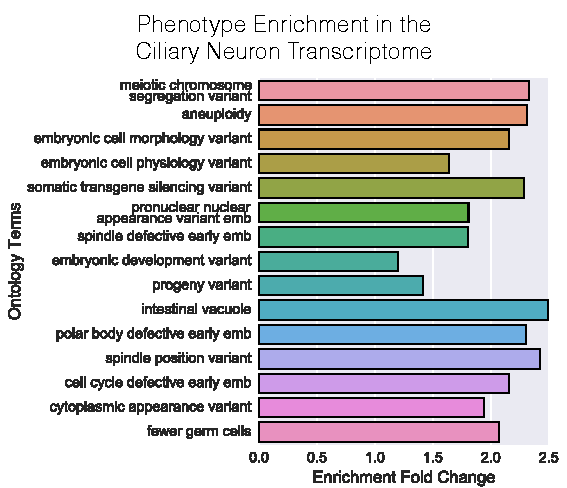
\includegraphics[width=\linewidth]{ciliary-transcriptome.pdf}
  \caption{PEA shows that the ciliary transcriptome is enriched in phenotypes
  related to cell division. Although this could reflect enrichment of
  microtubules and microtubule-related genes, the enrichment is at least
  partially driven by cell-cycle and DNA repair genes.}
\label{fig:cilia}
\end{figure}


In addition, TEA points at the \cel{} gonad primordium, the somatic gonad
and early embryonic cells as the sites where genes associated with ciliary neurons
are enriched. The `male distal tip cell' is a tissue
that is overrepresented in this dataset, but `distal tip cell' is not enriched.
In \cel{} the hermaphrodite distal tip cells (DTCs) and the male DTC are very
similar to each other in their biological functions (both maintain a stem cell
niche in the distal gonad). However, the male DTC is non-migratory, whereas the
hermaphrodite DTCs are migratory. Therefore, the term `male distal tip cell'
may reflect cellular aspects that are correlated with the non-migratory aspects
of the DTC biology, such as maintenance of proliferation.

Although one interpretation of the results would be that microtubule genes
are driving the enrichment of these terms, another possibility is that
there are cell-cycle genes that are driving the enrichment of these phenotypes
and tissues. Indeed, GO enrichment shows terms such as `DNA replication' (29
genes, \qval{5}), and `purine NTP-dependent helicase activity'
(15 genes, \qval{1}). Visual inspection of list in question reveals that
cell-cycle and DNA replication/repair genes are abundant in this transcriptome
and include genes such as \emph{atm-1}, \emph{dna-2}, or \emph{hpr-17}. This
analysis reveals that the ciliary neuron transcriptome is enriched in
genes associated with microtubules, but includes genes that are thought to
interact with DNA either via repair mechanisms or cell-cycle
control~\cite{Hofmann2000,Lee2003a,Bailly2010}.

\subsection*{Deconstructing phenotype-tissue relationships}
\subsubsection*{Tissue enrichment on the Egl gene set reveals cellular
components of the phenotype}
How does a phenotype emerge? We realized that with the tools that we have
developed, it is possible to understand what tissues contribute to a phenotype
in a probabilistic framework. In other words, we can extract all genes associated
with a particular phenotype, then search for tissue terms that are enriched to
understand how a phenotype arises from interactions between anatomical regions.
As a test of this, we selected the egg-laying defective (Egl) phenotype.
In \cel{}, egg-laying is a complex behavior that involves
a large number of tissues~\cite{Li1990}. The somatic gonad acts as a
repository for the eggs,
the uterine seam cells help protect the uterus, and a variety of muscles help
contract the uterus and open the vulva to lay an egg~\cite{Sulston1977}. The
vulva must be well-formed
to allow passage of an egg, and the hermaphrodite-specific neuron (HSN) is involved
in the egg-laying control~\cite{Schafer2005}. The complexity of the interactions that
happen to allow egg-laying make understanding the Egl phenotype in terms of
tissues a challenging task.

We extracted all of the \cel{} genes that have been associated with an Egl
phenotype and we used TEA to understand what tissues are enriched. The HSN
was enriched more than five-fold above background (\qval{7}) as were vulD, vulC,
vulE and vulF (\qval{6}). The vulA, vulB2 and vulB1 were
enriched at slightly lower levels (\qval{5}), whereas the uterine muscles and
uterine seam cells were enriched more than twice above background levels
(\qval{2}) (see Fig.~\ref{fig:egl}).
Therefore, the Egl phenotype would seem to emerge primarily from defects in the
HSN, secondarily from defects in the vulva, and only sometimes from defects in the
uterine seam cells or muscles. It is notable that all vulval cells were not equally
enriched. Although all the `vul' cells are annotated to a similar degree (between
50--70 genes for each cell type), the vulD and vulC cells had the largest
enrichment effect size and the lowest q-values, suggesting that these cells
are more likely to be associated with an Egl phenotype than the others. This may
reflect the fact that vulD and vulE are the site of attachment for four vulval
muscles, vm1. Perhaps this attachment is particularly fragile, and perturbations
to these cells prevent adequate function of these muscles. In support of these
observations, P7.pa had the largest fold-enrichment of any tissue. In \cel{},
P7.pa gives rise to vulD and vulC. However, vulF is
also attached to a set of four additional vulval muscles, vm2. Why
is vulF less associated with an Egl phenotype?

\begin{figure}[htbp]
  \renewcommand{\familydefault}{\sfdefault}\normalfont{}
  \centering
  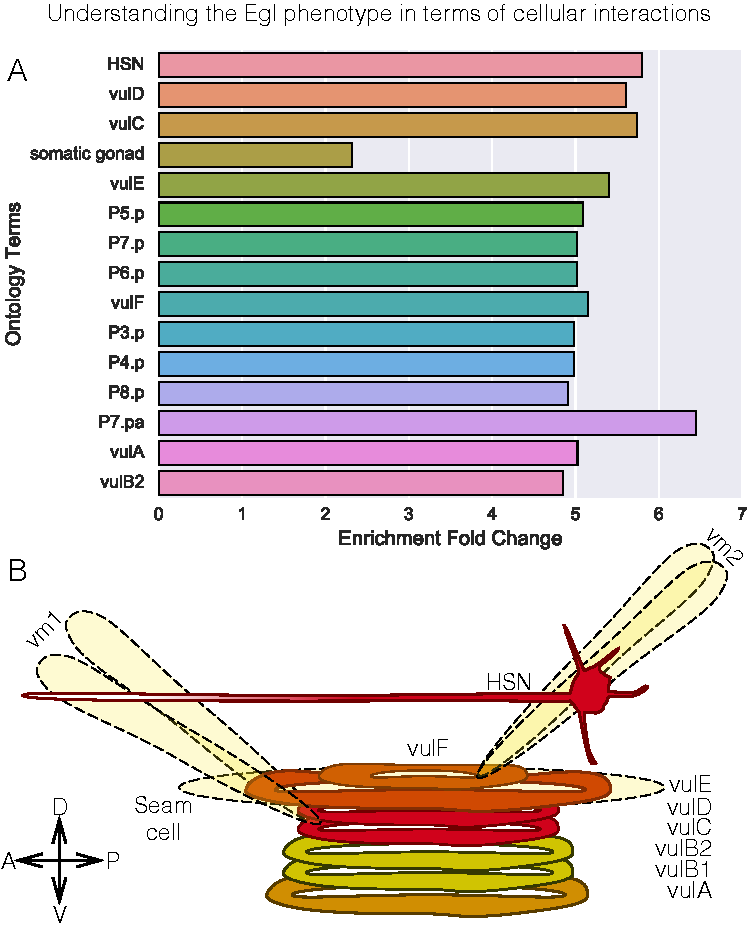
\includegraphics[width=\linewidth]{Egl-phenotype.pdf}
  \caption{The Egl phenotype is a complex phenotype that is the result of
  interactions between many tissues. To dissect the contributions of individual
  tissues to generating an Egl phenotype, we obtained all genes annotated with
  with an Egl term. \textbf{A} We used TEA on the set of Egl genes to identify
  enriched tissues. \textbf{B} Anatomic diagram showing the tissues that are
  most enriched in the Egl gene set. Color coding shows the qualitative
  ordering of enrichment (red-Most enriched, yellow-least enriched). For clarity,
  not all cells are shown. All vm1 (4 cells) and vm2 (4 cells) muscles are
  symmetrical arranged around the vulva, but only 2 cells are shown for each.
  There are two seam cells on the left and right side of the vulva, but only
  cell on the right is shown. Only terminally differentiated cells are shown.}
\label{fig:egl}
\end{figure}


\subsubsection*{Quantifying the anatomy-phenotype
                mapping via Bayesian probabilities}
Another way to understand the phenotype-anatomy mapping is by considering
how informative a given anatomy term is on a particular phenotype, or vice-versa.
To this end, we calculated two conditional probabilities that helped us answer
this question. The first conditional probability,

\begin{equation}
  P( \text{a gene has Egl annotation} | \text{it is expressed in } X)
\end{equation}

answers the question: For a gene with an expression pattern that includes the
tissue term X (i.e., the gene is expressed at least in X), what is the probability
that this gene has an Egl phenotype (i.e., the phenotype annotations for this
gene include Egl)? For simplicity, we can re-write this equation more succintly
by removing a few words. The calculation of this probability is straightforward
and follows from the definition of conditional probability:

\begin{equation}
  P(\text{Egl}|X) = \frac{N_\text{genes annotated Egl and X}}
                         {N_\text{genes annotated with X}}.
\label{egl_x}
\end{equation}

Equation~\ref{egl_x} measures how likely a gene is to be annotated with an Egl
phenotype given that its expression pattern includes the term $X$. A related
quantity (which is neither the inverse nor the complement) is the conditional
probability that a gene which is annotated with at least the Egl phenotype is
expressed in tissue $X$. That is to say,

\begin{equation}
  P(X|\text{Egl}) = \frac{N_\text{genes annotated Egl and X}}
                         {N_\text{genes annotated with Egl}}.
  \label{x_egl}
\end{equation}

Equation~\ref{x_egl} tells us how probable it is that any given gene that is
annotated with an Egl phenotype includes $X$ as a tissue term. Taken together,
equations~\ref{egl_x} and~\ref{x_egl} help us understand how predictive
anatomic expression is of phenotypes, and how predictive phenotypes are of
anatomic expression.

\begin{table*}
  \renewcommand{\familydefault}{\sfdefault}\normalfont{}
  \centering{}
  \ra{1.3}
  \caption{Conditional probabilities for various tissues. The
  first column shows the conditional probability that a gene has an Egl
  phenotype given that it has expression in tissue $X$ (given by the row).
  The second column shows the conditional probability that a gene has expression
  in the anatomy term X given that it has an Egl phenotype. The first 9 terms
  are the terms for which $P(\text{Egl}|X)$ is maximized. The last three terms
  are the terms which have the highest $P(X|\text{Egl})$. For clarity, the Pn.p
  cells are not shown even though $P(\text{Egl}|\text{Pn.p})\sim 0.24$.}

  \begin{tabular}{@{}lcc@{}}
  \toprule{}
  Tissue & $P(\text{Egl}| X)$ & $P(X|\text{Egl})$\\
  \bottomrule{}\\
  % Data goes here
  P7.pa & $0.30$ & $0.04$\\
  HSN & $0.27$ & $0.11$\\
  vulC & $0.27$ & $0.06$\\
  vulD & $0.26$ & $0.07$\\
  vulE & $0.25$ & $0.06$\\
  vulF & $0.24$ & $0.06$\\
  vulA & $0.24$ & $0.05$\\
  vulB2 & $0.23$ & $0.05$\\
  vulB1 & $0.22$ & $0.05$\\
  nervous system & $0.02$ & $0.72$ \\
  pharynx  & $0.00$ & $0.46$\\
  sex organ & $0.07$ & $0.41$\\
  tail & $0.05$ & $0.33$\\
  \bottomrule{}
  \end{tabular}
\label{tab:cond_probs}
\end{table*}

We calculated the conditional probability that a gene has an Egl phenotype given
that it's expression pattern includes a tissue term $X$ and we searched for the
tissue terms that maximized this probability. The list of terms that maximized this
probability reflected the results from running TEA on the subset of genes that have
an Egl phenotype. We also calculated the conditional probability that a gene has
expression in a tissue term $X$ given that it is annotated with an Egl phenotype
and we searched for terms that maximized this probability (see
Table~\ref{tab:cond_probs}). The terms that maximized this probability were
`nervous system', `pharynx' (a body part with a lot of neurons),
`sex organ' and `tail' (a body part with neurons and hypodermis). In general, the
terms that had a high $P(\text{Egl}|X)$ did not have a high $P(X|\text{Egl})$.
Additionally, the terms that had a high $P(X|\text{Egl})$ are broad terms that
include a lot of cells, whereas the terms that had a high $P(\text{Egl}|X)$
were considerably more specific.
We conclude that the Egl phenotype arises from a small set of tissues. The Egl
phenotype can be best predicted by genes with expression patterns that include
at least one of a small number of cells (mainly vul cells, HSN). On the other
hand, answering whether the expression pattern of a gene includes a particular
anatomic region or tissue given that the gene has an Egl phenotype is hard to
do for small tissues or single cells. However, guesses about what functional system
or broad anatomic region an Egl gene is expressed in can be answered with
confidence ($\sim70\%$ of the time, an Egl mutant is expressed in
the nervous system).

\section*{Conclusions}
The addition of GO and Phenotype Ontology enrichment testing to WormBase marks
an important step towards a unified set of analyses that can help researchers
to understand genomic datasets. These enrichment analyses will allow the community to
fully benefit from the data curation ongoing at WormBase. By using the same
algorithms to generate enrichment dictionaries for testing and using the
same model to test for term enrichment, these tools provide a coherent framework
with which to analyze genomic data. In particular, it is our hope that
phenotype enrichment will be of use to geneticists performing genome-wide
analyses, because they are familiar with the ontological terms that are tested
and with their biological meaning. Ideally, PEA could allow researchers to
design better screens to maximize target gene identification by quantifying
the phenotypes that are most overrepresented. An intriguing new direction of
research would be to create a controlled language for screening methods. With
such a language, we should be able to computationally suggest to a researcher
what screens one may wish to perform given a dataset.



\bibliography{pea-citations}
\bibliographystyle{pnas2011}


\end{document}
